\documentclass[../main]{subfiles}

%TeXromancers title page template
%by derivada.schwarziana

\begin{document}

%please update these for each book release:

\newcommand{\bookauthor}{J. F. Adams}
\newcommand{\shortbookauthor}{Adams}
\newcommand{\booktitle}{Stable Homotopy and Generalised Homology}
\newcommand{\booksubtitle}{}

\newcommand{\bookcoverTeXromancers}{Revised and modernized edition by}

\newcommand{\bookcoverpicture}{
\adjustbox{scale=0.75,center}{
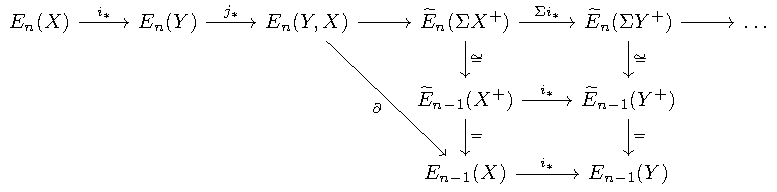
\includegraphics[height=15em]{./figure/ch9fig1_edited.pdf}}
}

\newcommand{\bookoriginaledition}{1974} % ?
\newcommand{\bookthisedition}{2022}

%these are meant for the back cover
%both should have ~100 words
\newcommand{\bookreview} 
{J. F. Adams, the founder of stable homotopy theory, gave a lecture series at the University of Chicago in 1967, 1970, and 1971, the well-written notes of which are published in this classic in algebraic topology. The three series focused on Novikov’s work on operations in complex cobordism, Quillen’s work on formal groups and complex cobordism, and stable homotopy and generalized homology. Adams’s exposition of the first two topics played a vital role in setting the stage for modern work on periodicity phenomena in stable homotopy theory. His exposition on the third topic occupies the bulk of the book and gives his definitive treatment of the Adams spectral sequence along with many detailed examples and calculations in KU-theory that help give a feel for the subject. 
}

\newcommand{\bookauthorbio}
{\emph{J. F. Adams} (1930-1989) was born in Woolwich, London. He received his Ph.D. from the University of Cambridge in 1956. His thesis, written under the supervision of Shaun Wylie, was titled \emph{On spectral sequences and self-obstruction invariants}.
\\[1em]

Adams was a pioneer in the field of stable homotopy theory. The Adams spectral sequence is one of the most important computational tools in the field. He used this to classify the division algebras over $\bR$. He also invented Adams operations in $K$-theory, and used it to solve the famous vector fields on spheres problem.

Adams received a lot of awards for his work. To list a few: the Sylvester Medal of the Royal Society of London in 1982, the 1963 junior Berwick Prize and the 1974 Senior Whitehead Prize from The London Mathematical Society
}

\newcommand{\authorbiosource}{U.Chicago press, \emph{MacTutor History of Mathematics Archive}; \emph{Mathematics Genealogy Project}}
%\newcommand{\aboutandlegal}{} %UNUSED -- blurb about what the group is and maybe mention legal stuff in back cover    %BOOK INFO GOES HERE -- please update _BOOKINFO.tex for new books
%http://paletton.com/#uid=b14333r0kkAw01RZWclMishq8B4eb

\definecolor{tyellow}{HTML}{FFD05B}
\definecolor{tyellowlight}{HTML}{FFE39D}
\definecolor{tyellowlighter}{HTML}{FFFBF0}
\definecolor{tyellowdark}{HTML}{D09B18}
\definecolor{tyellowdarker}{HTML}{715000}

\definecolor{tturq}{HTML}{3EAF7F}
\definecolor{tturqlight}{HTML}{86DAB6}
\definecolor{tturqlighter}{HTML}{EEFCF6}
\definecolor{tturqdark}{HTML}{118F59}
\definecolor{tturqdarker}{HTML}{004D2C}

\definecolor{tblue}{HTML}{3E83A1}
\definecolor{tbluelight}{HTML}{86BCD4}
\definecolor{tbluelighter}{HTML}{EEF8FC}
\definecolor{tbluedark}{HTML}{156283}
\definecolor{tbluedarker}{HTML}{033247} %colors

%title page
\newpage
\thispagestyle{empty}


\begin{tikzpicture}[remember picture,overlay]
%uses the calc library
    \node (title)
        [shape=rectangle, 
         outer sep=2em,
         inner sep=2em,
         minimum height=18em, 
         minimum width=\paperwidth, 
         align=flush right, 
         text=black,
         text width=0.8\paperwidth,
         anchor=north
        ] 
        at ($(current page.center)!0.6!(current page.north)$)
        {
        \fontsize{5em}{4em}
        \fontfamily{lmss}
        \selectfont
        \booktitle\par
        };
        
    \node (author)
        [
         inner sep=0.75em,
         align=flush right,
         text=black,
         anchor=east
        ]
        at ($(title.north east)-(0.125\paperwidth,0)$)
        {
        \fontsize{3em}{2.5em}
        \fontfamily{lmss}
        \selectfont
        \bookauthor\par
        };
    \node (coverinfo)
        [text=black]
        at ($(current page.center)!0.825!(current page.south)$)
        {
        \fontsize{1.5em}{1em}
        \fontfamily{lmss}
        \selectfont
        \bookcoverTeXromancers\par
        };
    \node
        [text=black]
        at ($(current page.center)!0.9!(current page.south)$)
        {
        
\includegraphics[height=3em]{texromancers_gray.pdf}
        \raisebox{1.1em}{
        \fontsize{1.5em}{1em}\selectfont\TeX{}romancers\par
        }
        };
\end{tikzpicture}

\end{document}